\subsubsection{2018.10.26组会}
\label{sec:g2018:1026}
\bhei{出席人员}:\RenZH、\TangLT、\ZY、\ZhangYX

\bhei{记录}:\RenZH、\ZY

\sect{工作情况}
\begin{itemize}
\item \RenZH:
    \begin{itemize}
        \item 概率编程模型的目的:
            \begin{itemize}
                \item 能够降低对专业能力的要求。
                \item 缩短开发时间,提高代码可读性。
                \item 优化运行的效率,减少开销。
            \end{itemize}
        \item 介绍Infer.Net提供的基本API:Variable的声明,使用,Inference Engine的使用。
        \item 通过图1,说明Infer.Net模型构建的思路,即 模型-> C\#代码 -> .Net程序。
            \begin{figure}[h]
                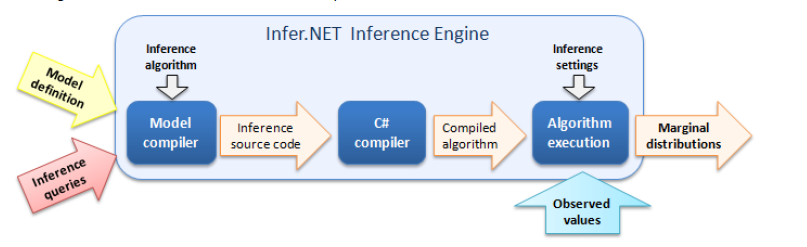
\includegraphics[width=\linewidth]{pic/how_work}
                \caption{Infer.Net模型}
            \end{figure}
        \item 关于这个项目的想法:
            \begin{itemize}
                \item 用某个概率编程模型开发一个机器学习应用并比较和其他方式构建的区别。
                \item 设计一个基于某个语言的概率编程工具。
            \end{itemize}
        \item 收集到的资料集。
    \end{itemize}
\item \TangLT:
    \begin{itemize}
        \item 概率编程模型的概念和目的。
        \item Pymc介绍。
        \item 通过例子介绍Pymc能做的事情。
        \item Pymc的其他功能。
        \item 一些可参考的书。
            \begin{figure}[h]
                
\includegraphics[scale=0.2]{pic/books}
                \caption{参考书}
            \end{figure}
        \item 贝叶斯推断,隐含马尔科夫模型重要性和地位。
        \item Pymc的一些局限和思考。
    \end{itemize}
\redt{Q1.OpenQASM问题}:量子编程模型中处理不确定性和概率编程中的相似点。

\end{itemize}

\sect{下步工作建议}
\begin{itemize}
\item \RenZH:
    \begin{itemize}
    \item 根据一个已经投入使用的,应用了概率编程模型的开源项目,看它使用的模型构建过程,不必过度关注算法,而是考虑这样的项目对于概率编程模型有什么要求,目前概率编程模型还有什么缺陷。
    \item 浏览Infer.Net的API文档,考虑其中设计的道理,总结其中体现的思想。
    \item 做一个已经有了的应用并没有太大意义,目前的精力还是需要放在模型构建本身上。
    \end{itemize}
\item \TangLT:
    \begin{itemize}
        \item 根据Pymc的API文档,考虑其中设计的道理,总结其中体现的思想。
        \item 一起讨论Infer.Net和Pymc的设计区别和其中的动机。
        \item 既然要填充算法的设计者和编程之间的隔阂,就应该让模型隐藏更多的编程细节,体现更多数学的思想。
    \end{itemize}
\end{itemize}

\sect{讨论达成的共识}

\begin{itemize}
    \item 概率编程模型主要用在构建机器学习的模型中。
    \item 目前主要的方式还是构建抽象层次比较高的API来完成。
    \item 概率编程最重要的任务是简化模型的表示。
\end{itemize}

\sect{还需要讨论的问题}

概率编程模型最佳的构建起点是什么,目前还是一些代码性的描述,是否需要更直观和数学化的方式进行描述?